% ------------------------------------------------------------------------------
% TYPO3 CMS 7.6 - What's New - Chapter "In-Depth Changes" (French Version)
%
% @author	Patrick Lobacher <patrick@lobacher.de> and Michael Schams <schams.net>
% @license	Creative Commons BY-NC-SA 3.0
% @link		http://typo3.org/download/release-notes/whats-new/
% @language	French
% ------------------------------------------------------------------------------
% LTXE-CHAPTER-UID:		7229f1b9-b481e9bc-09c46183-a86b6a7e
% LTXE-CHAPTER-NAME:	In-Depth Changes
% ------------------------------------------------------------------------------

\section{Changements en profondeur}
\begin{frame}[fragile]
	\frametitle{Changements en profondeur}

	\begin{center}\huge{Chapitre 3~:}\end{center}
	\begin{center}\huge{\color{typo3darkgrey}\textbf{Changements en profondeur}}\end{center}

\end{frame}

% ------------------------------------------------------------------------------
% LTXE-SLIDE-START
% LTXE-SLIDE-UID:	aea49b86-3243ab21-f5e10246-ce839567
% LTXE-SLIDE-ORIGIN:	159a2d7f-b679989c-30cf1736-6693f827 English
% LTXE-SLIDE-TITLE:		Bootstrap for Install Tool (1)
% ------------------------------------------------------------------------------

\begin{frame}[fragile]
	\frametitle{Changements en profondeur}
	\framesubtitle{Bootstrap pour l'Install Tool (1)}

	\begin{itemize}

		\item L'Install Tool utilise maintenant Bootstrap - pour l'installation~:

			\begin{figure}
				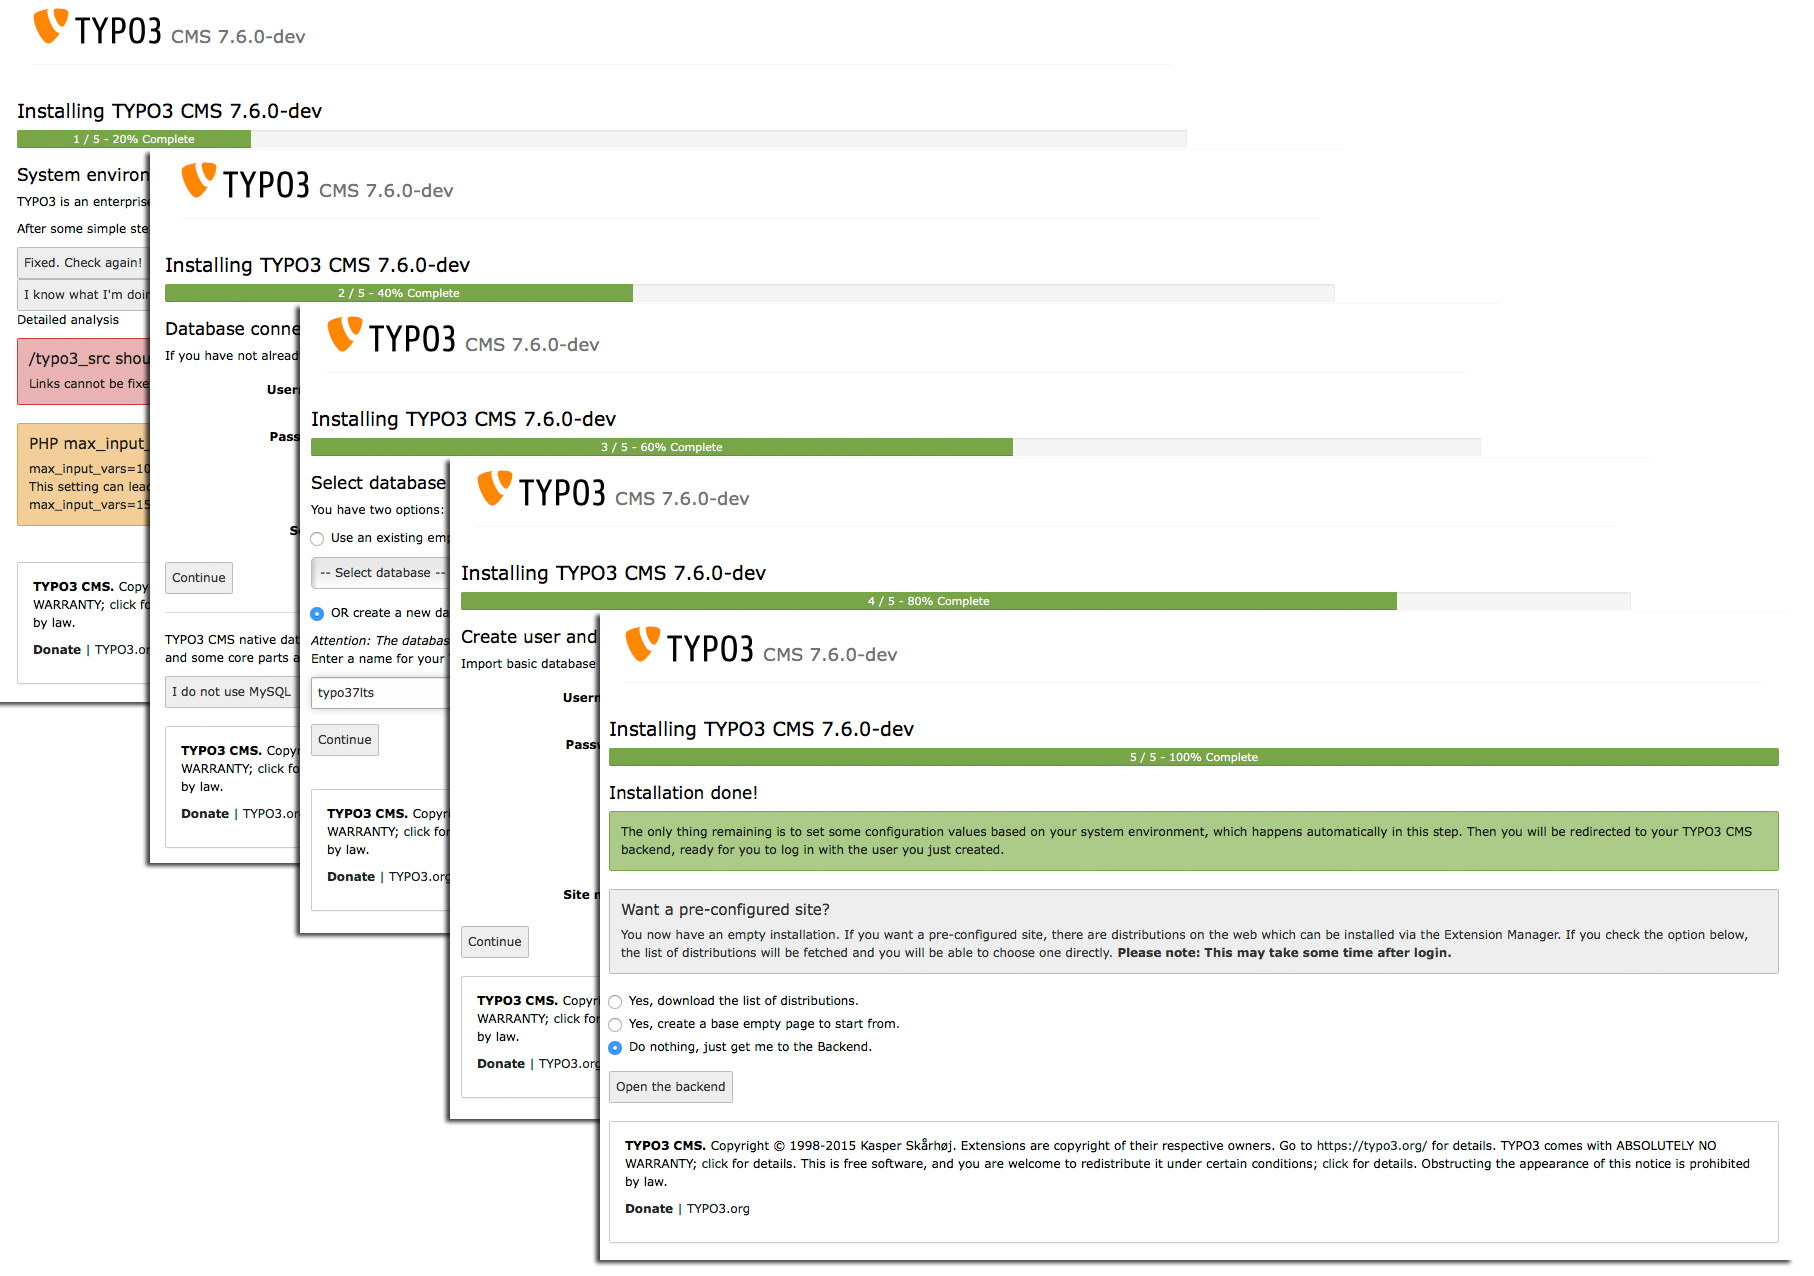
\includegraphics[width=0.7\linewidth]{InDepthChanges/InstallToolBootstrap01.jpg}
			\end{figure}

	\end{itemize}

\end{frame}

% ------------------------------------------------------------------------------
% LTXE-SLIDE-START
% LTXE-SLIDE-UID:		8c701b00-a15fd68b-b015062a-1c08c7c6
% LTXE-SLIDE-ORIGIN:	66a71f73-91b6c90e-e548a037-e2d47f94 English
% LTXE-SLIDE-TITLE:		Bootstrap for Install Tool (2)
% ------------------------------------------------------------------------------

\begin{frame}[fragile]
	\frametitle{Changements en profondeur}
	\framesubtitle{Bootstrap pour l'Install Tool (2)}

	\begin{itemize}

		\item L'Install Tool utilise maintenant Bootstrap - pour la configuration~:

			\begin{figure}
				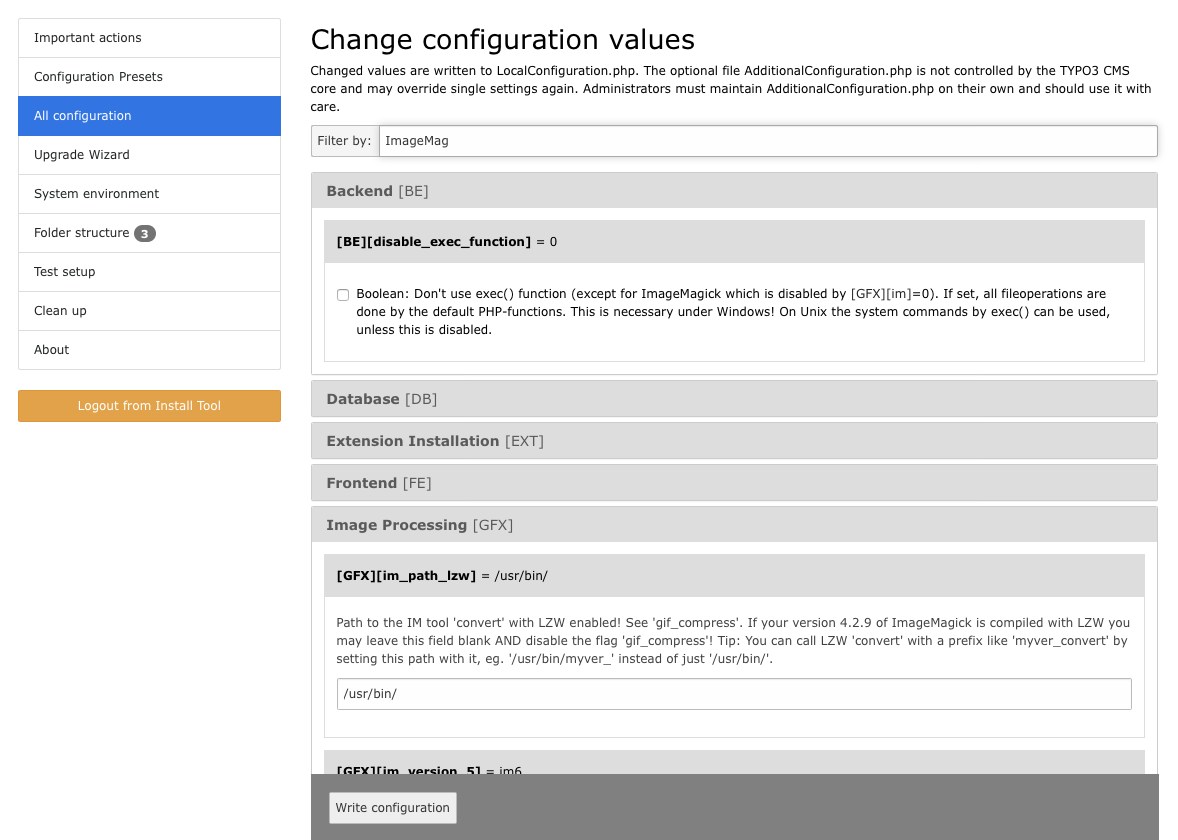
\includegraphics[width=0.7\linewidth]{InDepthChanges/InstallToolBootstrap02.png}
			\end{figure}

	\end{itemize}

\end{frame}

% ------------------------------------------------------------------------------
% LTXE-SLIDE-START
% LTXE-SLIDE-UID:		bd66fd18-3df4908e-f2620542-ccaee388
% LTXE-SLIDE-ORIGIN:	f901074a-4080140f-dd93e505-1e8c2178 English
% LTXE-SLIDE-ORIGIN:	d5acb2d2-159a2d7f-6693f827-30cf1736 German
% LTXE-SLIDE-TITLE:		Form protection API for frontend usage
% LTXE-SLIDE-REFERENCE:	Feature-56633-FormProtectionAPIForFrontEndUsage.rst
% ------------------------------------------------------------------------------

\begin{frame}[fragile]
	\frametitle{Changements en profondeur}
	\framesubtitle{Protection CSRF pour les plugins Frontend}

	% decrease font size for code listing
	\lstset{basicstyle=\tiny\ttfamily}

	\begin{itemize}

		\item Une nouvelle classe permet l'usage de l'API FormProtection en frontend

		\item Elle implémente la protection CSRF (Cross-Site Request Forgery)

			\begin{lstlisting}
				$formToken = \TYPO3\CMS\Core\FormProtection\FormProtectionFactory::get()->getFormProtection()->generateToken('news', 'edit', $uid);
				if (
				  $dataHasBeenSubmitted
				  && \TYPO3\CMS\Core\FormProtection\FormProtectionFactory::get()->validateToken(
				    \TYPO3\CMS\Core\Utility\GeneralUtility::_POST('formToken'), 'User setup', 'edit')) {
				  // processes the data
				}
				else {
				  // invalid token!
				}
			\end{lstlisting}

	\end{itemize}

\end{frame}

% ------------------------------------------------------------------------------
% LTXE-SLIDE-START
% LTXE-SLIDE-UID:		ba3e9763-7c60bd47-93a9f66c-511f3ffe
% LTXE-SLIDE-ORIGIN:	0198b067-68da7843-6a6d3f6d-94cee9b7 English
% LTXE-SLIDE-ORIGIN:	388c7243-b679989c-e2b30dbb-78f1aea4 German
% LTXE-SLIDE-TITLE:		Added LinkBrowser APIs (1)
% LTXE-SLIDE-REFERENCE:	Feature-66369-AddedLinkBrowserAPIs.rst
% ------------------------------------------------------------------------------

\begin{frame}[fragile]
	\frametitle{Changements en profondeur}
	\framesubtitle{Onglets pour l'explorateur de liens (1)}

	% decrease font size for code listing
	\lstset{basicstyle=\tiny\ttfamily}

	\begin{itemize}

		\item Il est possible d'étendre l'explorateur de liens (LinkBrowser) avec de nouveaux onglets

		\item Chaque onglet est pris en charge par un gestionnaire de lien (LinkHandler),
			devant implémenter l'interface suivante~:\newline
			\small
				\texttt{\textbackslash TYPO3\textbackslash CMS\textbackslash Recordlist\textbackslash LinkHandler\textbackslash LinkHandlerInterface}
			\normalsize

		\item Les gestionnaires sont enregistrés en TSconfig de page comme suit~:

			\begin{lstlisting}
				file {
				  handler = TYPO3\\CMS\\Recordlist\\LinkHandler\\FileLinkHandler
				  label = LLL:EXT:lang/locallang_browse_links.xlf:file
				  displayAfter = page
				  scanAfter = page
				  configuration {
				    customConfig = passed to the handler
				  }
				}
			\end{lstlisting}

	\end{itemize}

\end{frame}

% ------------------------------------------------------------------------------
% LTXE-SLIDE-START
% LTXE-SLIDE-UID:		ac72a41e-057b5276-78d7c233-9449b80b
% LTXE-SLIDE-ORIGIN:	7ff322bc-2ace574c-34ddebb5-559fd90c English
% LTXE-SLIDE-ORIGIN:	dfd89b4b-7b4b816c-e5904ba8-2527339b German
% LTXE-SLIDE-TITLE:		Added LinkBrowser APIs (2)
% LTXE-SLIDE-REFERENCE:	Feature-66369-AddedLinkBrowserAPIs.rst
% ------------------------------------------------------------------------------

\begin{frame}[fragile]
	\frametitle{Changements en profondeur}
	\framesubtitle{Onglets pour l'explorateur de liens (2)}

	% decrease font size for code listing
	\lstset{basicstyle=\tiny\ttfamily}

	\begin{itemize}

		\item Les options \texttt{displayBefore} et \texttt{displayAfter} définissent la position de l'onglet

		\item Les options \texttt{scanBefore} et \texttt{scanAfter} définissent l'ordre dans lequel les
			gestionnaires sont exécutés lors de l'analyse des liens existants

			\begin{lstlisting}
				$GLOBALS['TYPO3_CONF_VARS']['SC_OPTIONS']['LinkBrowser']['hooks'][1444048118] = [
				  'handler' => \Vendor\Ext\MyClass::class,
				  'before' => [], // optional
				  'after' => [] // optional
				];
			\end{lstlisting}

	\end{itemize}

\end{frame}

% ------------------------------------------------------------------------------
% LTXE-SLIDE-START
% LTXE-SLIDE-UID:		4edb5b46-5d928797-a57acd21-908d2bc1
% LTXE-SLIDE-ORIGIN:	1ef90646-4f4342dd-3bf0112b-95acba1b English
% LTXE-SLIDE-ORIGIN:	687f24a3-032124a3-7ac41f15-26329962 German
% LTXE-SLIDE-TITLE:		Module Template API (1)
% LTXE-SLIDE-REFERENCE:	Feature-69814-ModuleTemplateAPI.rst
% ------------------------------------------------------------------------------

\begin{frame}[fragile]
	\frametitle{Changements en profondeur}
	\framesubtitle{Module Template API (1)}

	% decrease font size for code listing
	\lstset{basicstyle=\tiny\ttfamily}

	\begin{itemize}

		\item La nouvelle API de template des modules a pour but de normaliser l'implémentation de DocHeaders

		\item Exemple 1~: ajouter un bouton

			\begin{lstlisting}
				$openInNewWindowButton = $this->moduleTemplate->getDocHeaderComponent()->getButtonBar()
				  ->makeLinkButton()
				  ->setHref('#')
				  ->setTitle($this->getLanguageService()->sL(
				    'LLL:EXT:lang/locallang_core.xlf:labels.openInNewWindow', TRUE
				    ))
				  ->setIcon($this->iconFactory->getIcon('actions-window-open', Icon::SIZE_SMALL))
				  ->setOnClick($aOnClick);

				$this->moduleTemplate->getDocHeaderComponent()->getButtonBar()
				  ->addButton($openInNewWindowButton, ButtonBar::BUTTON_POSITION_RIGHT);
			\end{lstlisting}
	\end{itemize}

\end{frame}

% ------------------------------------------------------------------------------
% LTXE-SLIDE-START
% LTXE-SLIDE-UID:		a78ac855-026f59fc-25c02ac6-a7e6e100
% LTXE-SLIDE-ORIGIN:	44c8e88e-5668ccb6-3cf424ea-c6a40ecf English
% LTXE-SLIDE-ORIGIN:	1570c8c9-2dfa48e9-058d2d04-bff5465d German
% LTXE-SLIDE-TITLE:		Module Template API (2)
% LTXE-SLIDE-REFERENCE:	Feature-69814-ModuleTemplateAPI.rst
% ------------------------------------------------------------------------------

\begin{frame}[fragile]
	\frametitle{Changements en profondeur}
	\framesubtitle{Module Template API (2)}

	% decrease font size for code listing
	\lstset{basicstyle=\tiny\ttfamily}

	\begin{itemize}
		\item Exemple 2~: ajouter un menu avec un élément

			\begin{lstlisting}
				$languageMenu = $this->moduleTemplate->getDocHeaderComponent()
				  ->getModuleMenuRegistry()->makeMenu()
				  ->setIdentifier('_langSelector')
				  ->setLabel($this->getLanguageService()->sL(
				    'LLL:EXT:lang/locallang_general.xlf:LGL.language', TRUE
				  ));

				$menuItem = $languageMenu->makeMenuItem()
				  ->setTitle($lang['title'] . $newTranslation)
				  ->setHref($href);

				if((int)$lang['uid'] === $currentLanguage) {
				  $menuItem->setActive(TRUE);
				}

				$languageMenu->addMenuItem($menuItem);
				$this->moduleTemplate->getDocHeaderComponent()->getModuleMenuRegistry()->addMenu($languageMenu);
			\end{lstlisting}
	\end{itemize}

\end{frame}


% ------------------------------------------------------------------------------
% LTXE-SLIDE-START
% LTXE-SLIDE-UID:		e67bb8d1-7a11ef85-e66b9451-e4e04173
% LTXE-SLIDE-ORIGIN:	2ffbc623-117a44dc-923610ec-78a3afc2 English
% LTXE-SLIDE-ORIGIN:	df3ea848-d5406e98-edbd6684-485ff477 German
% LTXE-SLIDE-TITLE:		PSR-7-based Routing for Backend AJAX Requests
% LTXE-SLIDE-REFERENCE:	Feature-69916-PSR-7-basedRoutingForBackendAJAXRequests.rst
% ------------------------------------------------------------------------------

\begin{frame}[fragile]
	\frametitle{Changements en profondeur}
	\framesubtitle{Routage PSR-7 des requêtes AJAX du Backend}

	% decrease font size for code listing
	\lstset{basicstyle=\tiny\ttfamily}

	\begin{itemize}

		\item Pour ajouter une route pour une requête AJAX, le fichier
			\texttt{Configuration/Backend/AjaxRoutes.php}\newline
			doit être créé avec le contenu suivant~:

			\begin{lstlisting}
				return [
				  // do something
				  'unique_route_name' => [
				    'path' => '/toolcollection/some-action',
				    'target' => \Vendor\Controller\SomeController::class . '::myAction',
				  ]
				];
			\end{lstlisting}

	\end{itemize}

\end{frame}

% ------------------------------------------------------------------------------
% LTXE-SLIDE-START
% LTXE-SLIDE-UID:		c694e2d7-2d964128-faa3d8c4-964b50dd
% LTXE-SLIDE-ORIGIN:	b68a9d26-30e6d4a0-7bccecf2-ad1f93c6 English
% LTXE-SLIDE-ORIGIN:	cb01cca6-58e91977-d18fa0b3-cba021ab German
% LTXE-SLIDE-TITLE:		Introduced two new Hooks for OpenID (getUserRecord)
% LTXE-SLIDE-REFERENCE:	Feature-44127-HooksForOpenIdToAutomaticallyCreateUserAccounts.rst
% ------------------------------------------------------------------------------
\begin{frame}[fragile]
	\frametitle{Changements en profondeur}
	\framesubtitle{OpenID \texttt{getUserRecord} Hook}

	% decrease font size for code listing
	\lstset{basicstyle=\tiny\ttfamily}

	Deux hooks sont ajoutés au service OpenID (1/2)

		\begin{itemize}

			\item Hook 1~:\newline
				\smaller\smaller
					\texttt{\$GLOBALS['TYPO3\_CONF\_VARS']['SC\_OPTIONS']['openid']['getUserRecord']}
				\normalsize

				\begin{itemize}
					\item Permet de modifier l'enregistrement utilisateur après sa récupération,
					\item Ou de créer un nouvel enregistrement si aucun trouvé
					\item Reçoit les paramètres \texttt{record}, \texttt{response} et \texttt{authInfo}
				\end{itemize}

		\end{itemize}

\end{frame}

% ------------------------------------------------------------------------------
% LTXE-SLIDE-START
% LTXE-SLIDE-UID:		3f6e1659-874e7067-f442bdb4-80adf173
% LTXE-SLIDE-ORIGIN:	b9b259e4-9d35ace7-edff1014-7390d1d1 English
% LTXE-SLIDE-ORIGIN:	ea0bfed8-831666d7-1ba40bb9-7a95723a German
% LTXE-SLIDE-TITLE:		Introduced two new Hooks for OpenID (authRequest)
% LTXE-SLIDE-REFERENCE:	Feature-44127-HooksForOpenIdToAutomaticallyCreateUserAccounts.rst
% ------------------------------------------------------------------------------
\begin{frame}[fragile]
	\frametitle{Changements en profondeur}
	\framesubtitle{OpenID \texttt{authRequest} Hook}

	% decrease font size for code listing
	\lstset{basicstyle=\tiny\ttfamily}

	Deux hooks sont ajoutés au service OpenID (2/2)

		\begin{itemize}

			\item Hook 2~:\newline
				\smaller\smaller
					\texttt{\$GLOBALS['TYPO3\_CONF\_VARS']['SC\_OPTIONS']['openid']['authRequest']}
				\normalsize

				\begin{itemize}
					\item Permet de modifier la requête d'authentification avant qu'elle soit transmise
					\item Utilisable par exemple pour demander des attributs supplémentaires au serveur OpenID, comme un pseudonyme
					\item Reçoit les paramètres \texttt{authRequest} et \texttt{authInfo}
				\end{itemize}

		\end{itemize}

\end{frame}

% ------------------------------------------------------------------------------
% LTXE-SLIDE-START
% LTXE-SLIDE-UID:		f44983af-52802f9e-ad29b899-8320fdea
% LTXE-SLIDE-ORIGIN:	1626edc6-8d93ff84-f64178bf-8e7650df English
% LTXE-SLIDE-ORIGIN:	115a4459-3653bb99-1680d6ab-d8c3c69b German
% LTXE-SLIDE-TITLE:		Hook in BackendUserAuthentication::getDefaultUploadFolder (1)
% LTXE-SLIDE-REFERENCE:	Feature-68895-IntroducedHookInBackendUserAuthenticationgetDefaultUploadFolder.rst
% ------------------------------------------------------------------------------
\begin{frame}[fragile]
	\frametitle{Changements en profondeur}
	\framesubtitle{Hooks et Signals (1)}

	% decrease font size for code listing
	\lstset{basicstyle=\tiny\ttfamily}

	\begin{itemize}

		\item Le dossier d'envoi retourné par
			\texttt{BackendUserAuthentication::getDefaultUploadFolder()}
			peut être changé

		\item Le hook est inscrit dans le fichier \texttt{ext\_localconf.php} comme suit~:

			\begin{lstlisting}
				$GLOBALS['TYPO3_CONF_VARS']['SC_OPTIONS']['t3lib/class.t3lib_userauthgroup.php']
				  ['getDefaultUploadFolder'][] =
				  \Vendor\MyExtension\Hooks\DefaultUploadFolder::class . '->getDefaultUploadFolder';
			\end{lstlisting}

	\end{itemize}

\end{frame}

% ------------------------------------------------------------------------------
% LTXE-SLIDE-START
% LTXE-SLIDE-UID:		dfe5ddab-1bc9bf2b-fa1681f5-4318a0e8
% LTXE-SLIDE-ORIGIN:	9c150d50-ee3ba19b-120ef653-e714135c English
% LTXE-SLIDE-ORIGIN:	d1041967-32814ee3-2172e570-4a6d21bd German
% LTXE-SLIDE-TITLE:		Hook in BackendUserAuthentication::getDefaultUploadFolder (2)
% LTXE-SLIDE-REFERENCE:	Feature-68895-IntroducedHookInBackendUserAuthenticationgetDefaultUploadFolder.rst
% ------------------------------------------------------------------------------
\begin{frame}[fragile]
	\frametitle{Changements en profondeur}
	\framesubtitle{Hooks et Signals (2)}

	% decrease font size for code listing
	\lstset{basicstyle=\tiny\ttfamily}

	\small Exemple~:\normalsize

		\begin{lstlisting}
			<?php
			namespace Vendor\MyExtension\Hooks;
			use TYPO3\CMS\Core\Authentication\BackendUserAuthentication;
			use TYPO3\CMS\Core\Resource\Folder;

			/**
			 * Class DefaultUploadFolder
			 */
			class DefaultUploadFolder {

			  /**
			   * Get default upload folder
			   * If there is a folder present with the same name as the last part of the table name use that folder.
			   * @param array $params
			   * @param BackendUserAuthentication $backendUserAuthentication
			   * @return Folder
			   */
			   public function getDefaultUploadFolder($params, BackendUserAuthentication $backendUserAuthentication) {
			    [...]
		\end{lstlisting}

\end{frame}

% ------------------------------------------------------------------------------
% LTXE-SLIDE-START
% LTXE-SLIDE-UID:		c445c814-4f8d15af-01c56610-1a9dc2b9
% LTXE-SLIDE-ORIGIN:	a4d7bec0-6c19d8b2-6a6be951-5d5aa0c0 English
% LTXE-SLIDE-ORIGIN:	2f855107-2262065c-c865f953-91b4f0ea German
% LTXE-SLIDE-TITLE:		Hook in BackendUserAuthentication::getDefaultUploadFolder (3)
% LTXE-SLIDE-REFERENCE:	Feature-68895-IntroducedHookInBackendUserAuthenticationgetDefaultUploadFolder.rst
% ------------------------------------------------------------------------------
\begin{frame}[fragile]
	\frametitle{Changements en profondeur}
	\framesubtitle{Hooks et Signals (3)}

	% decrease font size for code listing
	\lstset{basicstyle=\tiny\ttfamily}

	\small Exemple (suite)~:\normalsize

		\begin{lstlisting}
			    [...]

			    /** @var Folder $uploadFolder */
			    $uploadFolder = $params['uploadFolder'];
			    $pid = $params['pid'];
			    $table = $params['table'];
			    $field = $params['field'];

			    $matches = [];
			    if (!empty($uploadFolder) && preg_match('/_([a-z]+)$/', $table, $matches)) {
			      $folderName = $matches[1];
			      if ($uploadFolder->hasFolder($folderName)) {
			        $uploadFolder = $uploadFolder->getSubfolder($folderName);
			      }
			    }
			    return $uploadFolder;
			  }
			}
		\end{lstlisting}

\end{frame}

% ------------------------------------------------------------------------------
% LTXE-SLIDE-START
% LTXE-SLIDE-UID:		1a1b925c-562071a9-e82c3639-b3de6ec5
% LTXE-SLIDE-ORIGIN:	2c656d9e-38b9be7a-d590cb6e-21eccd4d English
% LTXE-SLIDE-ORIGIN:	cd6ba83d-9f068dee-b8887ffa-4a2eff29 German
% LTXE-SLIDE-TITLE:		Diverse Änderungen
% LTXE-SLIDE-REFERENCE:	Deprecation-69822-DeprecateSelectFieldTca.rst
% ------------------------------------------------------------------------------
\begin{frame}[fragile]
	\frametitle{Changements en profondeur}
	\framesubtitle{Divers}

	\begin{itemize}

		\item L'usage du type de champ TCA \texttt{select} requière l'usage de l'option \texttt{renderType}

		\item Les valeurs valides sont~:

			\begin{lstlisting}
				'renderType' => 'selectMultipleSideBySide',
				'renderType' => 'selectCheckBox',
				'renderType' => 'selectSingle',
				'renderType' => 'selectSingleBox',
				'renderType' => 'selectTree',
			\end{lstlisting}

	\end{itemize}

\end{frame}

% ------------------------------------------------------------------------------
